\chapter*{Introduction}\addcontentsline{toc}{chapter}{Introduction}

%[Why do we need redshifts? cosmology problems and galaxy evolution, use as distance proxy via Hubble law]

Photometric redshift (\pz) estimation has been a staple of studies of galaxy evolution, large-scale structure, and cosmology since its conception decades ago \citep{Baum1962}.  
An extremely coarse spectrum in the form of photometry in a handful of broadband filters can be an effective substitute for the time- and photon-intensive process of obtaining a spectroscopic redshift (\sz), a procedure that may only be applied to relatively bright galaxies.  
Once the photometric colors are calibrated against either a library of spectral energy distribution (SED) templates or a data set of spectra for galaxies with known redshifts, a correspondence between photometric colors and redshifts may be constructed, forming a trustworthy basis for \pz\ estimation or testing.

Many more \pz s may be obtained in the time it would take to observe a smaller number of \sz s, and \pz s may be measured for galaxies too dim for accurate \sz\ confirmation, permitting the compilation of large surveys of galaxy redshifts spanning a broad range of redshifts and luminosities.  
\Pz s have thus enabled the era of precision cosmology, heralded by weak gravitational lensing tomography and baryon acoustic oscillation peak measurements.  
Calculations of correlation functions of cosmic shears and galaxy positions require large numbers of high-confidence redshifts of surveyed galaxies.  

However, \pz s are susceptible to inaccuracy and imprecision via a number of effects, particularly their inherent noisiness due to the coarseness of photometric filters, catastrophic errors in which galaxies of one type at one redshift are mistaken for galaxies of another type at a different redshift, and systematics introduced by observational techniques, data reduction processes, and training set limitations.  
The projection of these effects into the space of true and estimated redshifts is discussed extensively in \Chap{pzdc1}, and their impact on cosmological parameter constraints is addressed in \Chap{chippr}, and \Fig{fig:pedagogical_scatter} in particular.
Based on the goals of a photometric galaxy survey, requirements can be placed on the accuracy of \pz\ estimates.
For example, the Large Synoptic Survey Telescope (\lsst) states requirements for the main cosmological sample in the \lsst\ Science Requirements Document (SRD)\footnote{\url{https://docushare.lsstcorp.org/docushare/dsweb/Get/LPM-17}} and reproduced in \Tab{tab:lsst-srd}.

\begin{table}
	\begin{tabular}{ll}
		Number of galaxies & $\sim 10^{7}$\\
		Root-mean-square error & $\sigma_z < 0.02 (1+z)$\\
		$3 \sigma$ catastrophic outlier rate & $< 10\%$\\
		bias & $< 0.003$
	\end{tabular}
\tablabel{tab:lsstsrd}
\caption{\Pz\ requirements for \lsst\ cosmology.}
\end{table}

In addition to these limitations in accuracy, there is also the matter of uncertainty quantification; \pz s are often reported with presumed-Gaussian error bars derived without inclusion of all systematic errors, including the different selection effects between the photometric color- or magnitude-spaces of galaxies for which \pz s are desired and galaxies with \sz s are used to calibrate \pz\ estimators.
An example of the impact of this selection bias in the context of \citep[\project{zCOSMOS}][]{lilly_zcosmos_2009} and \citep[\project{COSMOS}][]{laigle_cosmos2015_2016} is shown in \Fig{fig:selection-bias}.
This lack of support can bias one-point statistics of the affected galaxy populations \citep{moresco_spot_2013}, and elaborate procedures for compensating for such bias have been developed in the context of two-point statistics of galaxy redshifts \citep{mandelbaum_precision_2008}.

\begin{figure*}
	\begin{center}
		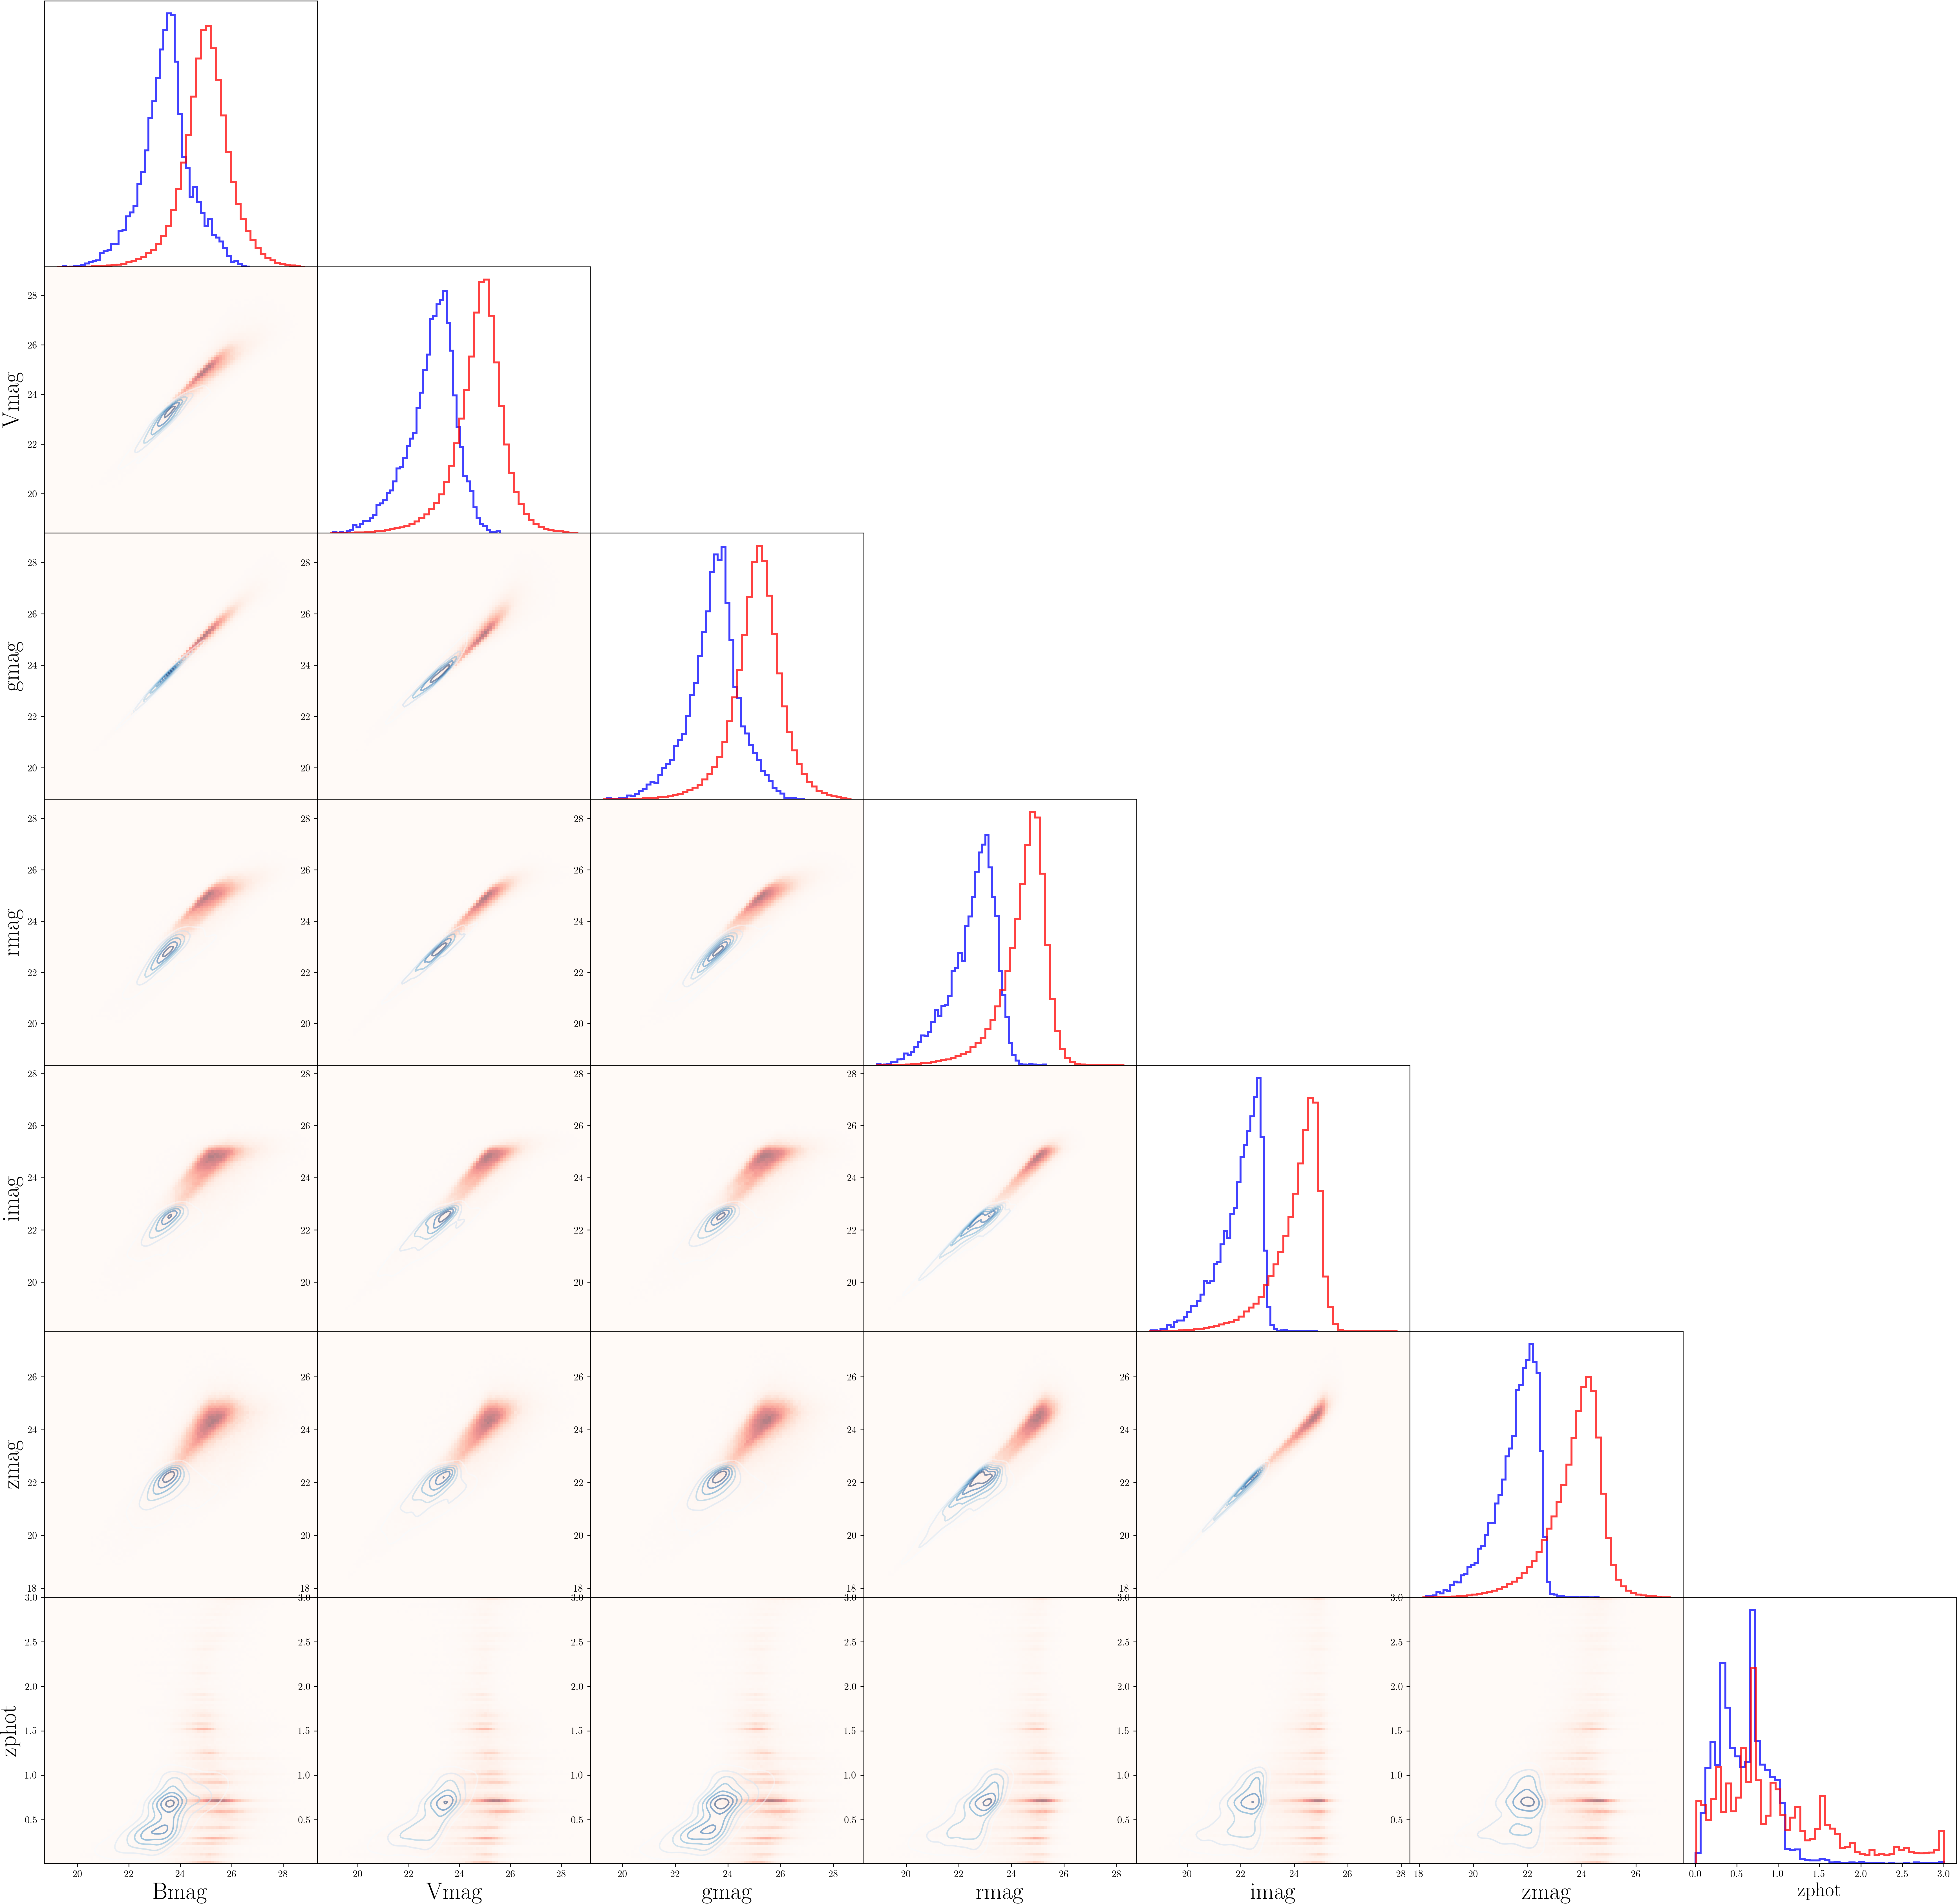
\includegraphics[width=0.99\textwidth]{figures/intro/big_corner_coarse.png}
		\caption{
			The distributions of magnitudes and the provided photometric redshift estimate for the galaxies with complete photometric data in \project{zCOSMOS} ($8,826$ galaxies; blue) and \project{COSMOS} ($395,019$ galaxies; red).
			It is evident that the sample for which spectra were unavailable is not well-supported by the sample for which spectra were obtained, which was used to calibrate the spectroscopically unconfirmed set.
		}
		\figlabel{fig:selection-bias}
	\end{center}
\end{figure*}

\aim{Hogg says ``I think it would be good to talk a little quantitatively about where people need to know N(z) and other one-point statistics, and how much they will get various things wrong if they don't know these correctly. 
	And situate that discussion within the current context of cosmological parameter estimation and precision cosmology.''}

%Several factors contribute to photometric redshifts' intrinsic scatter.  
%Distant galaxies are dimmer compared to galaxies of identical luminosity that are closer, driving up photometric errors in flux-limited surveys.  
%The nature of the galaxy sample at higher redshifts also changes, meaning the generation of the photometric redshift posterior based on an a locally-calibrated SED template library or spectroscopically-confirmed training set is more likely to be inappropriate, leading to broader features.  
%In general, the galaxies that could not have been observed spectroscopically will have different and noisier photo-$z$ likelihoods than those that could fall into a spectroscopic training set (or spectroscopically derived template library).  
%This effect may be stronger for high-redshift galaxies.  

Once propagated through the calculations of correlation functions of cosmic shear and galaxy positions, these sources of \pz\ errors are not insignificant contributors to the total uncertainties reported on cosmological parameters.
As other systematic errors have been resolved, the uncertainties associated with \pz s have come to dominate the uncertainties on estimates of cosmological parameters made by current surveys such as \citep[\des][]{hoyle_dark_2017}.

Much effort has been dedicated to improving \pz s, though they are still most commonly obtained by a maximum likelihood estimator (MLE) based on libraries of galaxy SED templates, with conservative approaches to error estimation.  
Recent advances have focused on identifying and removing catastrophic outliers when using \pz s for 
inference \citep{Gorecki2014}.  
Sophisticated Bayesian techniques and cutting-edge machine learning methods have been employed to improve precision \citep{Carliles2010} and accuracy \citep{Sadeh2015}. 

An alternative to point estimation of \pz s is redshift probability distribution function (PDF) estimation that reports the probability $p(z)$ over all possible redshifts for every galaxy rather than an MLE (with or without presumed Gaussian error bars) \citep{Koo1999}.  
This option is favorable because it contains more potentially useful information about the uncertainty on each galaxy's redshift than a point estimate, incorporating notions of precision, accuracy, and systematic errors.
However, denoting \pzpdf s as ``$\pr{z}$'' is an abuse of notation, as it does not adequately convey what information is being used to constrain the redshift $z$; \pzpdf s are \textit{posterior} PDFs, conditioned on the photometric data and prior knowledge, as is covered in detail in \Chap{pedant}, as well as \Chap{chippr} and \Chap{pzdc1}.

\aim{what interesting problems/opportunities are the context for my work?  (drawing conclusions about the universe from vast quantities of uncertainty-dominated, limitations of photometry lead to methodological challenges, what was tried so far and why isn't it good enough)}

\aim{what science can be done with that opportunity? (cosmology, and then some! the interesting problems are in testing LCDM, GR, inflation, also galaxy evolution)}

\Pzpdf s have been produced by completed surveys \citep{Hildebrandt2012, Sheldon2012} and will be produced by ongoing and upcoming surveys \citep{LSSTScienceCollaboration2009, CarrascoKind2014a, Bonnett2015, Masters2015}.  
\Pzpdf s are not without their own weaknesses, however, including the resources necessary to calculate and record them for large galaxy surveys \citep{CarrascoKind2014} and the method used to derive them.  
The most important of these issues, however, is that use of them in the literature is inconsistent at best and incorrect at worst.  
The most common application of \pzpdf s is their use in estimating \Nz, the distribution of redshifts of a sample of galaxies, a quantity essential to the calculation of the power spectra of weak gravitational lensing and large-scale structure that are used to constrain the parameters of cosmological models.
\aim{Provide equations/citations for the use of \Nz\ in cosmology.}

If the true redshifts $\{z_{j'}\}$ were known, the redshift probabilities would be delta functions $\{\delta(z, z'_{j})\}$ centered at the true redshift, and the redshift distribution could be approximated by a histogram or other interpolation of the delta functions $\{\delta(z, z'_{j})\}$.
When \pzpdf s are available instead of true redshifts, the simplest approach reduces them to point estimates of redshift by using $\delta(z, \hat{z}_{j})$ in place of $\delta(z, z'_{j})$, where $\hat{z}_{j}$ may be the mode (maximum) of the \pzpdf, though there are other, more principled options \citep{tanaka_photometric_2018-1}.
However, it is more common at this point to calculate the mathematically invalid but conceptually simple \textit{stacked estimator} of the redshift density function \citep{Lima2008}, 
\begin{align}
\eqlabel{eqn:stack}
\hat{n}(z) &= \frac{1}{\ntot} \sum_{i = 0}^{\ntot} \pr{z_{i}}
\end{align}
for a sample of $\ntot$ galaxies $i$, or, equivalently, the redshift distribution function $\hat{N}(z) = \ntot \hat{n}(z)$.

In \Chap{pedant}, I address the question of how a blatantly incorrect estimator of the redshift distribution could become widely accepted by otherwise clever astrophysicists.
I approach the problem from a mathematically rigorous perspective to identify the assumptions necessary for the stacked estimator to approach the true \Nz and note that because those assumptions will not hold for future surveys, including \lsst, we must use an alternative estimator that self-consistently propagates redshift uncertainty.

I go on to present one such an alternative to stacking, the Cosmological Hierarchical Inference with Probabilistic Photometric Redshifts (\Chippr), in \Chap{chippr}.
\Chippr\ is a probabilistic graphical model (PGM) that encapsulates the causal relationships between the redshift distribution, samples of individual galaxy redshifts, and photometric data.
I also present the \chippr\ code that implements the \Chippr\ model and includes a comprehensive suite of tools for testing arbitrarily realistic mock \pzpdf\ catalogs.

In order for the approach proposed in \Chap{chippr} to be applied, there must be a \pzpdf\ catalog, yet many techniques to obtain \pzpdf s have been proposed and tested in the literature without clear indications that one is superior to all others.  
An extension of the Bayesian photometric redshift (BPZ) method of \citet{Benitez2000} that produces posterior probability distributions (as opposed to a selection of local maxima) from an SED template library has been employed \citep{Hildebrandt2012, Kelly2014, Lopez-Sanjuan2015}.  
\Pzpdf s have also been obtained by a variety of trustworthy data-driven approaches in the literature: $k$-nearest neighbor algorithms with \citep{Ball2008} and without \citep{Sheldon2012} inclusion of photometric measurement errors, neural networks \citep{Bonnett2015a}, self-organizing maps \citep{CarrascoKind2014a}, and prediction tree and random forest classification techniques \citep{Carliles2010, CarrascoKind2013}.  
(The approaches of fitting to a training set and fitting to a template library are related to one another by \citet{Budavari2009}.)  

Hierarchical inference has also been applied to calculate \pzpdf s simultaneously with the overall redshift distribution function \citep{Leistedt2016}.  
Of course, this brief review does not cover all ways to obtain \pzpdf s; many more may be found in the literature, along with comparisons thereof \citep{Hildebrandt2010, Dahlen2013, Sanchez2013, Bonnett2015}.
Some current work aims to vet \pzpdf\ generation methods \citep{Wittman2016}.
\aim{Also cite the HSC comparison of \pzpdf\ methods, and maybe the DES one even though it only compares two.}
\Chap{pzdc1} details the comparative study of Schmidt, Malz, and Soo, et al. (in review) but goes beyond the scope of previous attempts to identify the best \pzpdf\ technique by critiquing the evaluation criteria themselves from a mathematically rigorous perspective.
\aim{Make this a real citation with a link to the paper.}

In the absence of an obvious best choice for the method used to derive \pzpdf s, \lsst\ has planned to provide \pzpdf s obtained by a number of promising methods rather than choosing one, effectively hedging their bets on which may ultimately prevail.
This goal of storing multiple \pzpdf s, however, must be accomplished without exceeding the available data storage capacity of the survey nor compromising the integrity of subsequent science applications due to loss of information in the compression and reconstruction schemes.
\Chap{qp} approaches the problem of choosing how best to store \pzpdf s such that the results of multiple \pzpdf\ techniques may be available to the scientific community, focusing in particular on the number of stored parameters under different possible parameterizations of stored \pzpdf s.

\aim{Update this paragraph for the existence of \Chap{pedant}.}
\Chap{chippr} presents a mathematically rigorous methodology for inferring \Nz\ from a catalog of \pzpdf s, including the effect of incorrectly inferred \Nz\ on cosmological parameter estimates.
\Chap{pzdc1} contains a comprehensive comparison of twelve approaches to probabilistic photometric redshift estimation, presenting novel discoveries of the impact of the assumptions implicit to the method by which the redshift probabilities are derived and the limitations of established performance metrics of such probabilistic data products in assessing the quality of the procedures for deriving them.
I also address in \Chap{qp} a practical concern regarding how redshift probabilities are to actually be used, answering the question of how probabilistic data products should be stored and delivered to users in order to ensure that scientific progress can be made, as well as how to go about answering that question for a generic science application.

\chapname~\chapalt{pedant} is original material developed initially as lecture notes and ultimately intended for submission to PRD.
\chapname~\chapalt{chippr} has been presented at numerous conferences and was awarded finalist status in the 2018 Dance Your Ph.D. Competition but remains a public draft \citep{malz_cosmological_2018} accompanied by the \chippr\footnote{\url{https://github.com/aimalz/chippr}} public code not yet submitted for publication.
\chapname~\chapalt{pzdc1} is currently under \desc\ internal review and publicly available online\footnote{\url{https://github.com/LSSTDESC/PZDC1paper}}, with intended submission to MNRAS.
\chapname~\chapalt{qp} has been refereed and published in AJ \citep{malz_approximating_2018}, and the \qp\footnote{\url{https://github.com/aimalz/qp}} code produced for the study is published \citep{malz_qp_2017}.

Here, I describe my specific contributions to each \chapname and acknowledge the contributions of my co-authors:
\begin{enumerate}

{\item For \chap{pedant}, I conducted the entire investigation, though Phil Marshall (SLAC) posed the initial question.}

{\item For \chap{chippr}, I led the development, implementation, and validation of \Chippr\ initially under the supervision of David Hogg (NYU) and later continued to work on all three aspects of the project under the supervision of Phil Marshall (SLAC).}

{\item For \chap{pzdc1}, I led the choice, evaluation, and interpretation of the comparison metrics, and I devised and implemented the \texttt{trainZ} technique of \pzpdf\ estimation.
	I wrote the paper in collaboration with Sam Schmidt (UC Davis), John Soo (U. of Science Malaysia), and the \Pz\ Working Group of the \desc.  
	The mock data was produced and validated by Alex Abate (Dia\&Co), Sam Schmidt (UC Davis), Eve Kovacs (Argonne), Joe DeRose (Stanford), Risa Wechsler (Stanford), Tina Peters (Toronto).
	The experimental design was chosen by Ofer Lahav (UCL), Jeff Newman (Pitt), Sam Schmidt (UC Davis), and Tony Tyson (UC Davis).
	I chose the metrics to test with input from Jeff Newman (Pitt) and Ann Lee (CMU).
	I worked together with Rongpu Zhou (Pitt), Bryce Kalmbach (UW), Kartik Iyer (Rutgers), Sam Schmidt (UC Davis), and Chris Morrison (UW) to implement the comparison metrics and run them on the results of different \pzpdf\ codes.
	The \pzpdf\ codes themselves were written and/or run by Ibrahim Almosallam (King Abdulaziz City for Science and Technology), Massimo Brescia (INAF-Capodimonte), Stefano Cavuoti (University Federico II), Johann Cohen-Tanugi (Universit\'e de Montpellier),  Andy Connolly (UW), Peter Freeman (CMU), Melissa Graham (UW), Rafael Izbicki (Federal University of Sao Carlos), Matt Jarvis (Oxford; University of the Western Cape), Ann Lee (CMU), Giuseppe Longo (University Federico II), Erfan Nourbakhsh (UC Davis), Eric Nuss (Universit\'e de Montpellier), Taylor Pospisil (CMU), Cecile Roucelle (U Clermont-Ferrand), and Hugo Tranin (Universit\'e de Montpellier).
	The paper is intended for submission to MNRAS but is still under internal review by \desc\ members Mike Troxel (Duke), Markus Michael Rau (CMU), and Daniel Gruen (Stanford).}

{\item For \chap{qp}, I devised the idea for the project, conducted the investigation, wrote and validated the \texttt{qp} code, and wrote the paper under the supervision of Phil Marshall (SLAC), with contributions to the mock data production by Sam Schmidt (UC Davis), Melissa Graham (UW), Joe DeRose (Stanford), and Risa Wechsler (Stanford).
	The paper was internally reviewed by \desc\ members Chad Schafer (CMU), Boris Leistedt (NYU), and Chris Morrison (UW).}

\end{enumerate}
